\chapter{Triple-Handshake RSA}
\label{chapter:RSA}

\section{Présentation}
\label{sec:pTHR}

L'attaque\up{\cite{article:handshake}} a été découverte par Antoine Delignat-Lavaud, Karthikeyan Bhargavan et Alfredo Pironti 
de l'équipe de recherche Prosecco de INRIA Paris-Rocquencourt. 

Elle est présentée comme une nouvelle classe d'attaque. Un client se connecte sur un serveur malicieux et le serveur
se connecte sur un serveur cible en se faisant passer pour le client. C'est une attaque MITM sur trois Handshake.
L'attaquant réussit l'attaque s'il réussit à se faire passer pour le client après la troisième poignée de main.


\section{Comment ça marche}
\label{sec:ccmTHR}

L'attaque se passe en trois étapes :

\subsection{Etape 1}
\label{sec:e1}

\begin{figure}[h]
\label{fig:hand1}
\centering
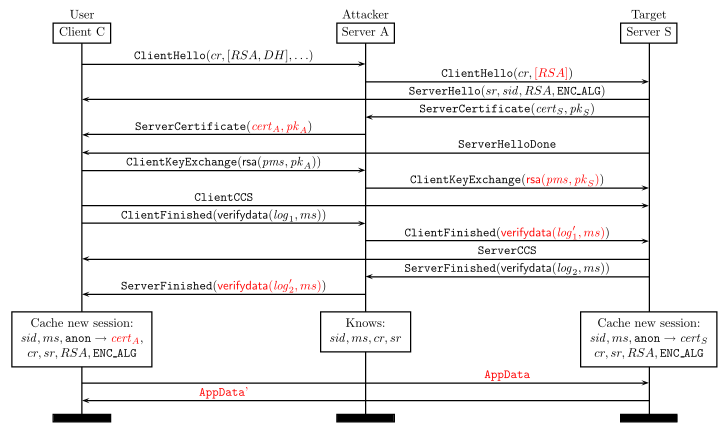
\includegraphics[scale=0.4]{Hand1}
\caption{Triple Handshake : Etape 1}
\end{figure}

Le client $C$ se connecte sur le serveur malicieux $A$. Dans le même temps, $A$ se connecte au serveur $S$ en utilisant
les informations de connexion de $C$. L'attaquant change la requête ClientHello pour imposer le choix de RSA. $A$
doit donner à $C$ et $S$ ses certificats.

$A$ va alors pouvoir récupérer le PMS ( Pre Master Secret ), et le réémettre au serveur. Il doit ensuite modifier
les logs. Ces messages sont les premiers à être chiffrés et contiennent un hashé de l'ensemble 
des messages échangés pendant la négociation. Il doit donc les modifier pour les faire correspondre au log de $C$ et $S$.

L'attaquant a deux connexions avec les mêmes paramètres et clés mais avec des certificats serveur et des logs 
différents. La première poignée de main est finie.

\subsection{Etape 2}
\label{sec:e2}

\begin{figure}[h]
\label{fig:hand2}
\centering
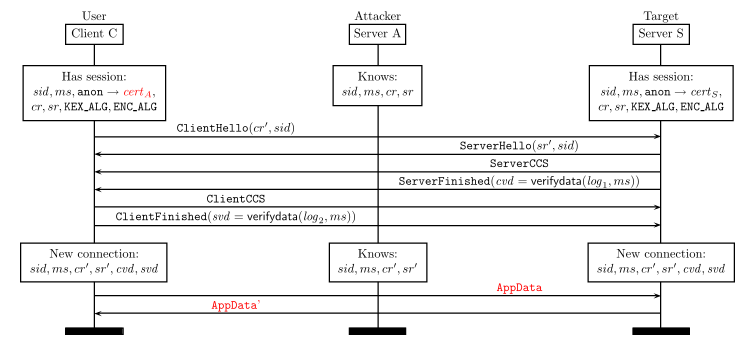
\includegraphics[scale=0.5]{Hand2}
\caption{Triple Handshake : Etape 2}
\end{figure}

$C$ se reconnecte à $A$ et demande un résumé de la connexion précédente. $A$ se reconnecte en retour à $S$ et demande la même chose.
Ensuite $A$ va seulement retransmettre les messages de $C$ vers $S$ et inversement.

A la fin de cette deuxième poignée de main, $C$ et $S$ ont maintenant les mêmes logs. Ils ont aussi négocié de
nouvelles clés, mais comme $A$ est au milieu, il les connait. 
\pagebreak

\subsection{Etape 3}
\label{sec:e3}

\begin{figure}[h]
\label{fig:hand3}
\centering
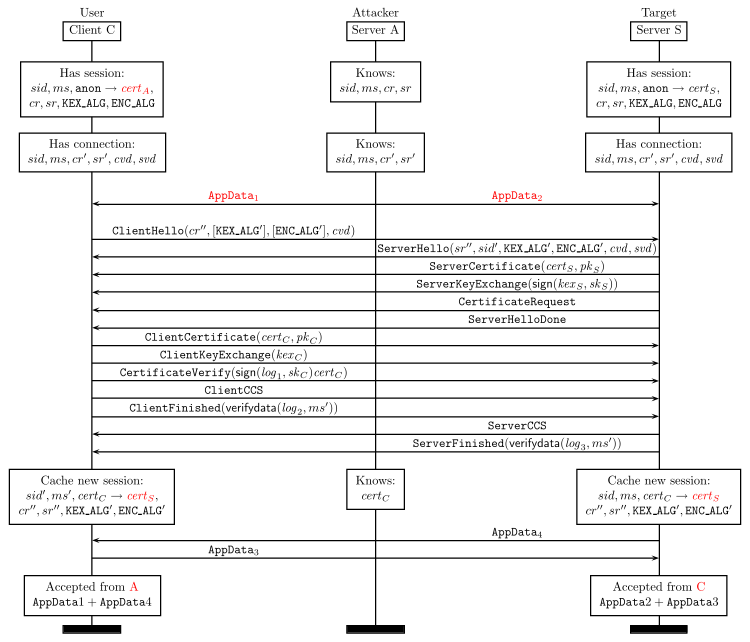
\includegraphics[scale=0.4]{Hand3}
\caption{Triple Handshake : Etape 3 }
\end{figure}

$S$ demande la renégociation complète avec authentification à $A$, qui envoie la demande à $C$. $A$ va seulement faire suivre les messages. A la
fin de la rénégociation, les données de connexion de $C$ et $S$ sont les mêmes. $S$ va envoyer son certificat à $C$.
En principe, $C$ devrait rejeter ce certificat mais en réalité il est accepté par de nombreux navigateurs. La raison
est simple, un serveur peut changer de certificat, parce qu'il a expiré par exemple.

Toutefois, $A$ n'a plus connaissance de la clé de session ou de la nouvelle master key. En effet, pour envoyer
le master secret, $C$ a utilisé la clé publique du certificat de $S$ donc $A$ ne peut pas la déchiffrer.
 Il ne peut donc pas agir ou observer les communications entre le client et le serveur. 

Cette vulnérabilité n'est pas exploitable seule. Cependant, $A$ peut par exemple retransmettre l'image exacte du site de $S$ en
y intégrant un script qui permet d'utiliser une attaque outrepassant le SOP.


\section{Contre-Mesures}
\label{sec:cmTHR}

Pour éviter ces attaques, il faudrait revoir la politique de TLS vis à vis du changement des certificats.
Il faudrait interdire de changer les certificats durant une renégociation. Ainsi la troisième étape ne 
fonctionnerait plus.

Une autre possibilité est de rajouter au master secret un hash du précédent handshake. Ainsi lors d'une
renégociation, le client et le serveur peuvent vérifier leur intégrité respective. Dans notre attaque, 
le hash sera éronné puisque $C$ aura l'identité de $A$ au lieu de $S$, de même pour $S$.

 

